\documentclass[border=5pt]{standalone}
\usepackage{tikz}
\usetikzlibrary{arrows.meta,calc}

\begin{document}
% Template: delayed adjustment path / J-curve
% Use for trade-balance J-curves, campaign wear-in, adoption lags,
% drawdown-and-recovery paths, and policy response lags.
% For trade/current-account J-curves, keep the timing order explicit:
% baseline before depreciation, immediate price-effect deterioration,
% trough after the event, then quantity adjustment and recovery.
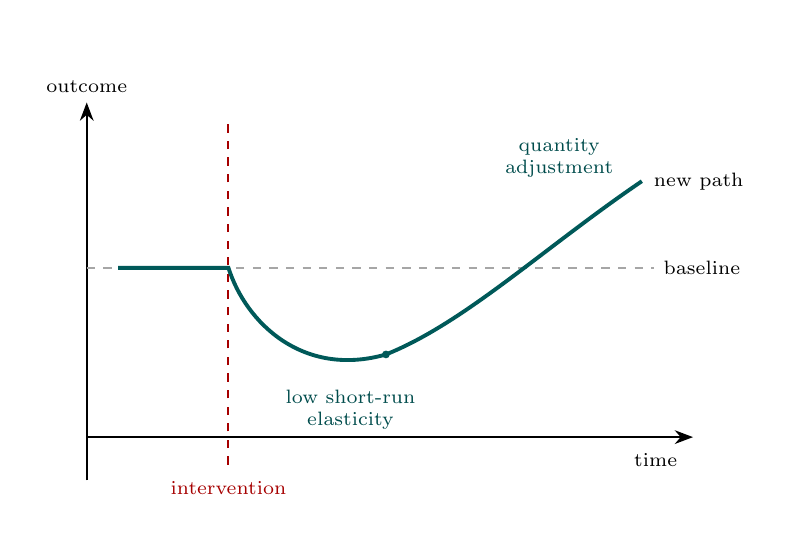
\begin{tikzpicture}[
  font=\sffamily,
  >=Stealth,
  axis/.style={->, line width=0.8pt},
  base/.style={draw=gray!70, dashed, line width=0.55pt},
  pathline/.style={draw=teal!70!black, line width=1.4pt},
  event/.style={draw=red!65!black, dashed, line width=0.7pt},
  lab/.style={font=\scriptsize, align=center},
  phase/.style={font=\scriptsize, align=center, text=teal!60!black}
]
\path[use as bounding box] (-0.75,-1.05) rectangle (8.75,5.2);

\draw[axis] (0,0) -- (7.7,0) node[below left=2pt, lab] {time};
\draw[axis] (0,-0.55) -- (0,4.25) node[above, lab] {outcome};
\draw[base] (0,2.15) -- (7.20,2.15) node[right, lab] {baseline};
\draw[event] (1.8,-0.35) -- (1.8,4.0);
\node[lab, text=red!65!black] at (1.8,-0.65) {intervention};

\draw[pathline]
  (0.4,2.15)
  .. controls (1.0,2.15) and (1.45,2.15) .. (1.8,2.15)
  .. controls (2.02,1.45) and (2.75,0.75) .. (3.8,1.05)
  .. controls (4.8,1.45) and (5.8,2.40) .. (7.05,3.25);

\fill[teal!70!black] (3.8,1.05) circle (1.4pt);
\node[phase] at (3.35,0.35) {low short-run\\elasticity};
\node[phase] at (6.00,3.55) {quantity\\adjustment};
\node[lab, anchor=west] at (7.08,3.25) {new path};
\end{tikzpicture}
\end{document}
